\documentclass[11pt]{article}

\usepackage[a4paper,margin=24mm]{geometry}
\usepackage[T1]{fontenc}
\usepackage{amsmath,amssymb,bm}
\usepackage{booktabs,longtable,tabularx,array}
\usepackage{graphicx}
\usepackage{xcolor}
\usepackage{enumitem}
\usepackage{hyperref}
\usepackage{url}

\hypersetup{
  colorlinks=true,
  linkcolor=blue!55!black,
  urlcolor=blue!55!black,
  citecolor=blue!55!black,
  pdftitle={Exact One-Electron Wilson Qualification in Aion},
  pdfauthor={Aion development record}
}
\setlist{nosep,leftmargin=*}
\setcounter{tocdepth}{2}
\renewcommand{\arraystretch}{1.16}
\emergencystretch=2em
\newcolumntype{Y}{>{\raggedright\arraybackslash}X}
\newcommand{\iu}{\mathrm{i}}
\newcommand{\dd}{\mathrm{d}}
\newcommand{\Tr}{\operatorname{Tr}}
\newcommand{\ReTr}{\operatorname{Re}\operatorname{Tr}}
\newcommand{\A}{\mathbf A}
\newcommand{\B}{\mathbf B}
\newcommand{\E}{\mathbf E}
\newcommand{\R}{\mathbf R}
\newcommand{\rvec}{\mathbf r}
\newcommand{\Smat}{\mathbf S}
\newcommand{\Kmat}{\mathbf K}
\newcommand{\omegamat}{\boldsymbol\omega_t}
\newcommand{\Dmat}{\mathbf D}
\newcommand{\Pmat}{\mathbf P}
\newcommand{\Gmat}{\mathbf G}
\newcommand{\filelink}[2]{\href{run:#2}{\texttt{#1}}}
\newcommand{\status}[1]{\textsf{#1}}

\title{\textbf{Exact One-Electron Wilson Qualification in Aion}\\
\large Physics, implementation, numerical evidence, and artifact index}
\author{Aion development record}
\date{19 September 2026}

\begin{document}
\maketitle

\begin{center}
\fbox{\begin{minipage}{0.92\textwidth}
\textbf{Qualification status.} Gates G0--G8 were explicitly reviewed and
accepted by the user.  The accepted scope is fixed-centre, linear,
one-electron straight-Wilson dynamics and the declared P0, E1, gB1, B1, and
C1 truncations on the tabulated fixtures.  The selected post-G8 branch is the
Aion adiabatic pure-LDA/GGA TDDFT closure.  That nonlinear closure is a future
branch and is not part of the evidence summarized here.
\end{minipage}}
\end{center}

\vspace{0.5em}
\noindent\textbf{Repository state represented by this report:}
\begin{center}
\texttt{feature/exact-one-electron-}\\
\texttt{wp7-action-observables}
\end{center}
The record begins from the accepted WP8 synthesis at commit \texttt{2fa0214}
and the subsequent review record.  Raw executions are immutable and retain
their execution-time status; acceptance is carried only by the separate files
in \texttt{docs/reviews}.

\tableofcontents
\listoffigures
\listoftables
\clearpage

\section{Purpose and how to use this report}

This document is the principal entry point to the exact one-electron Wilson
qualification campaign.  It has four jobs:

\begin{enumerate}
  \item state the physical and mathematical problem that was actually tested;
  \item describe the implemented evaluator, time connection, propagator, and
        action-derived observables;
  \item summarize the numerical results and the failed as well as accepted
        algorithmic explorations; and
  \item index the source code, plans, review decisions, raw executions,
        derived tables, figures, and verification tools needed to audit or
        reproduce every conclusion.
\end{enumerate}

The report deliberately distinguishes four kinds of statement:

\begin{description}[style=nextline]
  \item[Mathematical identity]
  A consequence of the declared continuum action, Wilson frame, and index
  conventions.  An identity may be true even before code exists.
  \item[Implemented feature]
  A reusable Aion code path.  Its existence alone does not show that it was
  executed in the accepted environment.
  \item[Executed numerical evidence]
  A hash-authenticated run or derived analysis tied to a repository commit,
  fixture, backend, precision, grid, and timestep.
  \item[Reviewed evidence]
  An explicit user decision in \texttt{docs/reviews}.  Only this level changes
  a gate to accepted.  Raw manifests remain \status{executed\_unreviewed}.
\end{description}

This distinction is especially important for WP6: the first time integrator
was implemented and executed but failed the declared model-difference
stability criterion.  The later mixed-index Gauss--Magnus experiment was then
implemented, executed to 128 intervals in the hard case, and accepted.

\section{Executive scientific conclusions}

\begin{enumerate}
  \item The direct dressed-orbital and endpoint-factorized routes reproduce
  the same exact straight-Wilson one-electron matrices at the measured
  quadrature floor.  Gauge-representative changes, gauge-origin changes,
  field reversal, pair reversal, and rigid rotation behave as required.
  \item P0 is a controlled small-field approximation only inside explicit
  system, basis, geometry, and operator brackets.  No molecule-independent P0 cutoff
  is supported by the data.
  \item The triangle-flux correction gB1 improves the overlap metric but does
  not supply the anchored-vector response required by the kinetic,
  nuclear-attraction, and total mechanical channels.  Full B1 resolves both
  onsite and offsite mechanical blocks.  Across the classified blocks, the
  median B1 error-reduction factor is 183.10.
  \item Multicentre loop flux makes the missing channels spectrally visible.
  In the cc-pVDZ above-threshold fixtures, P0 and gB1 can shift generalized
  eigenvalues by order-one to tens of hartree, whereas B1/C1 reduce the shift
  to roughly $3\times10^{-2}$--$4\times10^{-2}$ Ha.
  \item The natural mixed-index density $D=PS$ obeys an orthogonal-looking
  commutator equation even though the AO frame is nonorthogonal and moving.
  A fourth-order two-node Gauss--Magnus link with a $[2/2]$ Pad\'e exponential
  propagates it by similarity, without L\"owdin orthogonalization, endpoint
  Cholesky correction, or metric projection.
  \item The accepted 32/64/128-interval hard-case continuation measures global
  orders from 3.707 to 3.990.  The largest 64-to-128 change in a
  model-minus-exact density difference is 0.004454 of the final difference,
  below the declared 0.25 limit.
  \item In the distorted one-electron $\mathrm{H}_3^{2+}$ above-threshold
  pulse, only the complete first-order model C1 closely tracks the exact
  endpoint observables.  Its absorbed-energy difference is
  $2.2166\times10^{-7}$ Ha, compared with a timestep difference uncertainty
  of $7.95\times10^{-14}$ Ha; the residual is therefore a resolved model
  truncation difference, not a propagation artifact.
  \item Exact action derivatives give site charge, oriented-link current,
  weak continuum-current pairings, Ward identities, continuity, and uniform
  electric power.  On the finest accepted electric trajectory the integrated
  work defect is $-1.236\times10^{-9}$ Ha and the instantaneous action identity
  closes at $4.88\times10^{-16}$.
  \item CPU and physical-CuPy trajectories agree at approximately
  $1.5\times10^{-15}$--$4.1\times10^{-15}$ in the WP7 parity comparison.
\end{enumerate}

\section{Physical scope and terminology}

\subsection{Included}

The qualified problem uses finite molecules with fixed nuclei and fixed AO
anchors; real spherical Gaussian AOs from PySCF; straight paths from each
anchor to the electronic coordinate; local all-electron nuclear attraction;
prescribed electromagnetic sources; and no Maxwell backreaction.  Static
tests use uniform magnetic fields.  Dynamic tests use uniform electric fields
and a Maxwell-consistent time-dependent uniform magnetic field with its
affine induction electric field.

The pair campaign covers H--H, O--H, N$_2$, and CO; STO-3G, cc-pVDZ, and
aug-cc-pVDZ; bond-length scales 0.8, 1.0, and 1.25; and parallel,
perpendicular-$x$, perpendicular-$y$, and oblique field directions.  The
multicentre and dynamic fixtures use equilateral and distorted three-proton
frameworks.  Their electronic problem has one electron, so it is
$\mathrm{H}_3^{2+}$ and is a geometric qualification fixture, not a claim
about physical neutral H$_3$ or two-electron H$_3^+$.

\subsection{Excluded}

The accepted evidence does not cover self-consistent Hartree or XC feedback,
nonlinear SCEM propagation, moving nuclei or anchors, Pulay forces,
pseudopotentials, periodic systems, general nonuniform-field power balance,
Maxwell backreaction, or pointwise reconstruction of the continuum current
density.  Weak current pairings are source-covector tests, not a pointwise
current field.

\subsection{Meaning of ``exact''}

``EX'' or ``exact Wilson'' means the analytic pullback of the declared
one-electron action to the finite subspace spanned by the chosen
straight-Wilson-dressed Gaussian orbitals.  It is exact with respect to that
restriction, while retaining finite-basis and measured real-space quadrature
errors.  It is not an exact continuum Schr\"odinger solution.

\section{Wilson frame, restricted action, and approximation hierarchy}

\subsection{Electromagnetic and AO conventions}

In atomic units the electron has $q=-1$, $m=1$, and $\hbar=1$ in the executed
campaigns.  The covariant derivatives and physical fields are
\begin{align}
 D_t^\Phi &= \partial_t+\frac{\iu q}{\hbar}\Phi,
 &\boldsymbol\pi_{\A}&=-\iu\hbar\nabla-q\A,\\
 \E&=-\partial_t\A-\nabla\Phi,
 &\B&=\nabla\times\A.
\end{align}
The scalar-potential energy is carried by $D_t^\Phi$ and is not added again
to the mechanical energy.

For a bare real AO $e_\mu$ anchored at $\R_\mu$, define the straight-path
phase, Wilson factor, and dressed AO by
\begin{align}
 a_\mu[\A](\rvec,t)
 &=\int_0^1(\rvec-\R_\mu)\cdot
 \A(\R_\mu+s(\rvec-\R_\mu),t)\,\dd s,\\
 W_\mu&=\exp\!\left(\frac{\iu q}{\hbar}a_\mu\right),
 &\chi_\mu&=W_\mu e_\mu.
\end{align}
The coefficient density is $P=CfC^\dagger$ and lower matrices contract as
$\langle O\rangle=\ReTr(PO)$.  No extra closed-shell factor is inserted.

\subsection{Metric, connection, mechanical matrix, and equation of motion}

The exact projected metric, temporal connection, and one-electron mechanical
matrix are
\begin{align}
 S_{\mu\nu}&=\langle\chi_\mu|\chi_\nu\rangle,\\
 (\omega_t)_{\mu\nu}&=\langle\chi_\mu|D_t^\Phi\chi_\nu\rangle,\\
 K_{\mu\nu}&=\frac{1}{2m}
   \langle\boldsymbol\pi_\A\chi_\mu|\boldsymbol\pi_\A\chi_\nu\rangle
   +\langle\chi_\mu|v_{\rm nuc}|\chi_\nu\rangle.
\end{align}
They satisfy metric compatibility,
\begin{equation}
 \dot S=\omega_t+\omega_t^\dagger.
\end{equation}
The restricted real action yields
\begin{equation}
 \boxed{\iu\hbar\left(S\dot C+\omega_t C\right)=KC.}
\end{equation}
The ordinary-derivative matrix $K-\iu\hbar\omega_t$ is not the mechanical
energy.  This distinction prevents connection energy from being mislabelled
as an absorbed mechanical energy.

\subsection{Endpoint link and internal finite-spread geometry}

For the centre path from ket anchor $\R_\nu$ to bra anchor $\R_\mu$,
\begin{align}
 \Theta_{\mu\nu}
 &=\exp\!\left[\frac{\iu q}{\hbar}
   \int_{\R_\nu}^{\R_\mu}\A\cdot\dd\boldsymbol\ell\right],\\
 F^B_{\mu\nu}(\rvec)
 &=\Theta_{\mu\nu}^{-1}W_\mu(\rvec)^*W_\nu(\rvec).
\end{align}
$\Theta$ is an exact gauge-covariant endpoint link.  $F^B$ is the
gauge-invariant holonomy through the triangle formed by the two anchors and
$\rvec$.  With the anchored magnetic residual vector
\begin{equation}
 \mathbf C_\mu^B(\rvec)=\int_0^1s(\rvec-\R_\mu)\times
 \B(\R_\mu+s(\rvec-\R_\mu))\,\dd s,
\end{equation}
one has
$\boldsymbol\pi_\A\chi_\mu=W_\mu(-\iu\hbar\nabla+q\mathbf C_\mu^B)e_\mu$.
For a uniform $\B$, both $F^B$ and $\mathbf C_\mu^B$ are analytic affine
geometry factors.  Full matrices factor as the endpoint link times an
endpoint-removed internal amplitude, for example
$S=\Theta\odot\bar S$ and $K=\Theta\odot\bar K$.

The exact temporal connection follows from the electric line integral
\begin{equation}
 \mathcal V_\nu^E(\rvec,t)=\int_0^1(\rvec-\R_\nu)\cdot
 \E(\R_\nu+s(\rvec-\R_\nu),t)\,\dd s,
\end{equation}
as
\begin{equation}
 (\omega_t)_{\mu\nu}=\frac{\iu q}{\hbar}\Theta_{\mu\nu}
 \int \bar N_{\mu\nu}(\rvec,t)
 \left[\Phi(\R_\nu,t)-\mathcal V_\nu^E(\rvec,t)\right]\dd^3r.
\end{equation}
Thus the connection contains the anchor-scalar sector, endpoint-link motion,
and the internal electric finite-spread response.

\subsection{Comparison models}

Table~\ref{tab:model-hierarchy} gives the implemented action-consistent
hierarchy.  ``gB1'' means the geometric first magnetic correction only;
``B1'' includes the full first magnetic mechanical response; and ``C1'' is
the complete simultaneous first internal-amplitude order.

\begin{table}[htbp]
\centering
\caption{Action-level matrix content of each comparison model.}
\label{tab:model-hierarchy}
\begin{tabularx}{\textwidth}{lYYY}
\toprule
Model & Metric & Mechanical matrix & Temporal connection \\
\midrule
EX & exact & exact & exact \\
P0 & endpoint link $\times$ bare metric & endpoint link $\times$ bare mechanical matrix & P0-compatible connection \\
E1 & P0 & P0 & P0 plus internal electric increment \\
gB1 & full first magnetic metric & P0 & metric-compatible magnetic connection \\
B1 & full first magnetic metric & full first magnetic mechanical matrix & metric-compatible magnetic connection \\
C1 & full first magnetic metric & full first magnetic mechanical matrix & B1 connection plus internal electric increment \\
\bottomrule
\end{tabularx}
\end{table}

In the static electric-free sector C1 equals B1.  At zero magnetic curvature
and for a spatially uniform electric field, the exact connection reduces to
\begin{equation}
 \omega_t=\omega_{\rm P0}+\frac{\iu}{\hbar}V_{\rm E1},
 \qquad V_{\rm E1}=-\sum_\alpha E_\alpha D_\alpha,
\end{equation}
so the existing P0+E1 formulation is recovered in its declared domain.  E1
belongs in the connection; it is not an additional mechanical-energy term.

\section{Implementation architecture}

\subsection{How PySCF is used}

PySCF is the analytic and real-space electronic-structure backend, but it
does not determine the Wilson physics.  Aion uses it in four controlled ways:

\begin{enumerate}
  \item A \texttt{Mole} object fixes the geometry, real spherical AO basis,
  contractions, normalization, AO ordering, shell metadata, and AO-to-anchor
  map.  The occupancy-independent one-electron reference does not run RKS.
  \item Libcint supplies independent analytic zero-field overlap, kinetic,
  local nuclear-attraction, position, and canonical-momentum integrals.  These
  are both oracles and the zero-field analytic part of corrected finite-field
  contractions.
  \item PySCF atom-centred grids and AO evaluators supply values and first
  derivatives in deterministic blocks.  Aion applies Wilson triangle phases,
  anchored magnetic vectors, electric line integrals, and source variations
  before contracting the grid blocks.
  \item Exact finite-field results use ``analytic zero-field plus real-space
  finite-field correction''.  This prevents the complete matrix from
  inheriting the absolute zero-field quadrature error while retaining an
  independent raw-grid route for identity checks.
\end{enumerate}

The same blocked contractions run with NumPy or CuPy arrays.  Backend
residency is explicit; physical GPU tests verify that the CuPy path does not
silently fall back to host arrays.  GPU evidence applies to the qualified
matrix/propagation paths, not to an unimplemented nonlinear TDDFT closure.

\subsection{Reusable code map}

\begin{longtable}{p{0.32\textwidth}p{0.61\textwidth}}
\caption{Primary reusable implementation files.}\label{tab:code-map}\\
\toprule
File & Responsibility \\
\midrule
\endfirsthead
\toprule
File & Responsibility \\
\midrule
\endhead
\path{src/aion/electronic_structure/magnetic_matrices.py} & Exact static uniform-magnetic overlap, kinetic sectors, nuclear attraction, mechanical matrices, analytic first derivatives, direct-gauge oracle, and approximation hierarchy. \\
\path{src/aion/electronic_structure/time_connection.py} & Maxwell-consistent source samples; exact factorized and direct temporal connection; independently differentiated metric rate; electric, magnetic, and weak vector-potential source directions. \\
\path{src/aion/formulations/exact_one_electron.py} & EX/P0/E1/gB1/B1/C1 EOM triples; source directions; pure-gauge response; site charge, oriented-link current, continuity, electric power, and weak current pairings. \\
\path{src/aion/formulations/action.py} & Restricted one-electron action value and fixed-history, history, and full directional derivatives, with resolved metric, connection, and mechanical contractions. \\
\path{src/aion/propagation/tensorial.py} & Mixed/contravariant density conversion, complete generator, fourth-order Gauss--Magnus/$[2/2]$-Pad\'e link, similarity transport, and geometric diagnostics. \\
\path{src/aion/electromagnetism/test_variations.py} & Smooth localized Gaussian vector-potential variations and their straight-line integrals for weak continuum-current pairings. \\
\path{src/aion/io/transaction.py} & Transactional artifact writing used by authenticated campaign runners. \\
\bottomrule
\end{longtable}

The runner, analyzer, verifier, fixture, and test inventories are listed in
Appendices~\ref{sec:tool-index} and~\ref{sec:test-index}.  Those scripts are
campaign infrastructure; the physics and algorithms above live in reusable
\texttt{src/aion} modules.

\section{Evidence architecture and numerical error policy}

Each raw execution records the repository branch/commit/dirty state,
dependency versions, molecule and basis, AO metadata, grid policy and
fingerprint, electromagnetic representative and origin, model level,
precision/backend, tolerances, semantic array hashes, and raw residuals.
Typical immutable members are \texttt{execution\_plan.json},
\texttt{manifest.json}, \texttt{result.json}, \texttt{arrays.npz}, and
\texttt{completed.json}.  Derived analyses contain their own authenticated
summary, CSV tables, figures, and source hashes.

Numerical conclusions retain three separate scales:

\begin{itemize}
  \item the algebraic/roundoff residual;
  \item the real-space quadrature or basis refinement change; and
  \item the physical model-minus-reference difference.
\end{itemize}

A physical difference is not credited unless it is separated from the
appropriate numerical scale.  Field ``thresholds'' are sampled brackets: the
last tested point below a declared relative error and the first tested point
above it.  No interpolation or universal cutoff is implied.

\section{Static qualification: G0--G4}

\subsection{G0--G1: zero-field reference and quadrature floors}

The initial H--H/STO-3G checkpoint reconstructed overlap and weak-form kinetic
matrices on unpruned PySCF grids.  At grid level 4 (52,080 points), relative
Frobenius residuals against libcint were $1.5103\times10^{-11}$ for overlap
and $2.8208\times10^{-10}$ for kinetic energy.  G1 extended the test to O--H,
nuclear attraction, total mechanical energy, canonical momentum, levels
0--5, and NWChem pruning.

The accepted default is unpruned level 4; unpruned level 5 is the refinement;
NWChem-pruned level 4 is an alternative-pruning check.  The largest measured
level-5 working floor was the O--H canonical-momentum residual,
$2.21\times10^{-8}$, still roughly 450 times below the declared $10^{-5}$ grid
target.  Momentum-sign discrimination exceeded $9.4\times10^7$ for O--H and
$5.18\times10^9$ for H--H at level 4.

\subsection{G2: exact static Wilson evaluator}

For H--H/STO-3G at $|B|=0.08$ a.u., the maximum EX-direct/EX-link residual was
$5.70\times10^{-16}$.  Exact Gram matrices remained positive, with minimum
eigenvalue 0.3406818.  Symmetric/Landau representatives and two gauge origins
gave generalized-spectrum shifts no larger than $2.78\times10^{-16}$ Ha.
The O--H rigid-rotation fixture, including oxygen $p$-orbital mixing, gave a
maximum generalized-spectrum change of $2.42\times10^{-11}$ Ha, well below
the declared propagated tolerance.

\subsection{G3--G4: pair scan, first-order hierarchy, and channel attribution}

The accepted pair campaign contains 4 systems, 3 bases, 3 bond scales, 4
directions, both field signs where required, and field magnitudes from
$10^{-7}$ to 1 a.u.  The exact field data then serve as the parent for the
analytic first magnetic derivatives and finite-field remainder fits.

Figure~\ref{fig:validity-brackets} is the compact global view.  At relative
error $10^{-4}$, P0 is conservatively confirmed only through $10^{-4}$ a.u.
for all four matrix families.  gB1 extends overlap to
$3.162\times10^{-3}$ a.u. but leaves the other families at $10^{-4}$ a.u.
B1/C1 extend overlap, kinetic, and mechanical to
$3.162\times10^{-3}$ a.u. and nuclear attraction to $10^{-2}$ a.u.  At the
$10^{-2}$ error level the corresponding conservative brackets are $10^{-2}$
for P0; $3.162\times10^{-2}$ for gB1 overlap; and
$3.162\times10^{-2}$ for B1/C1 overlap, kinetic, and mechanical, with nuclear
attraction confirmed through $0.1$ a.u.

\begin{figure}[htbp]
\centering
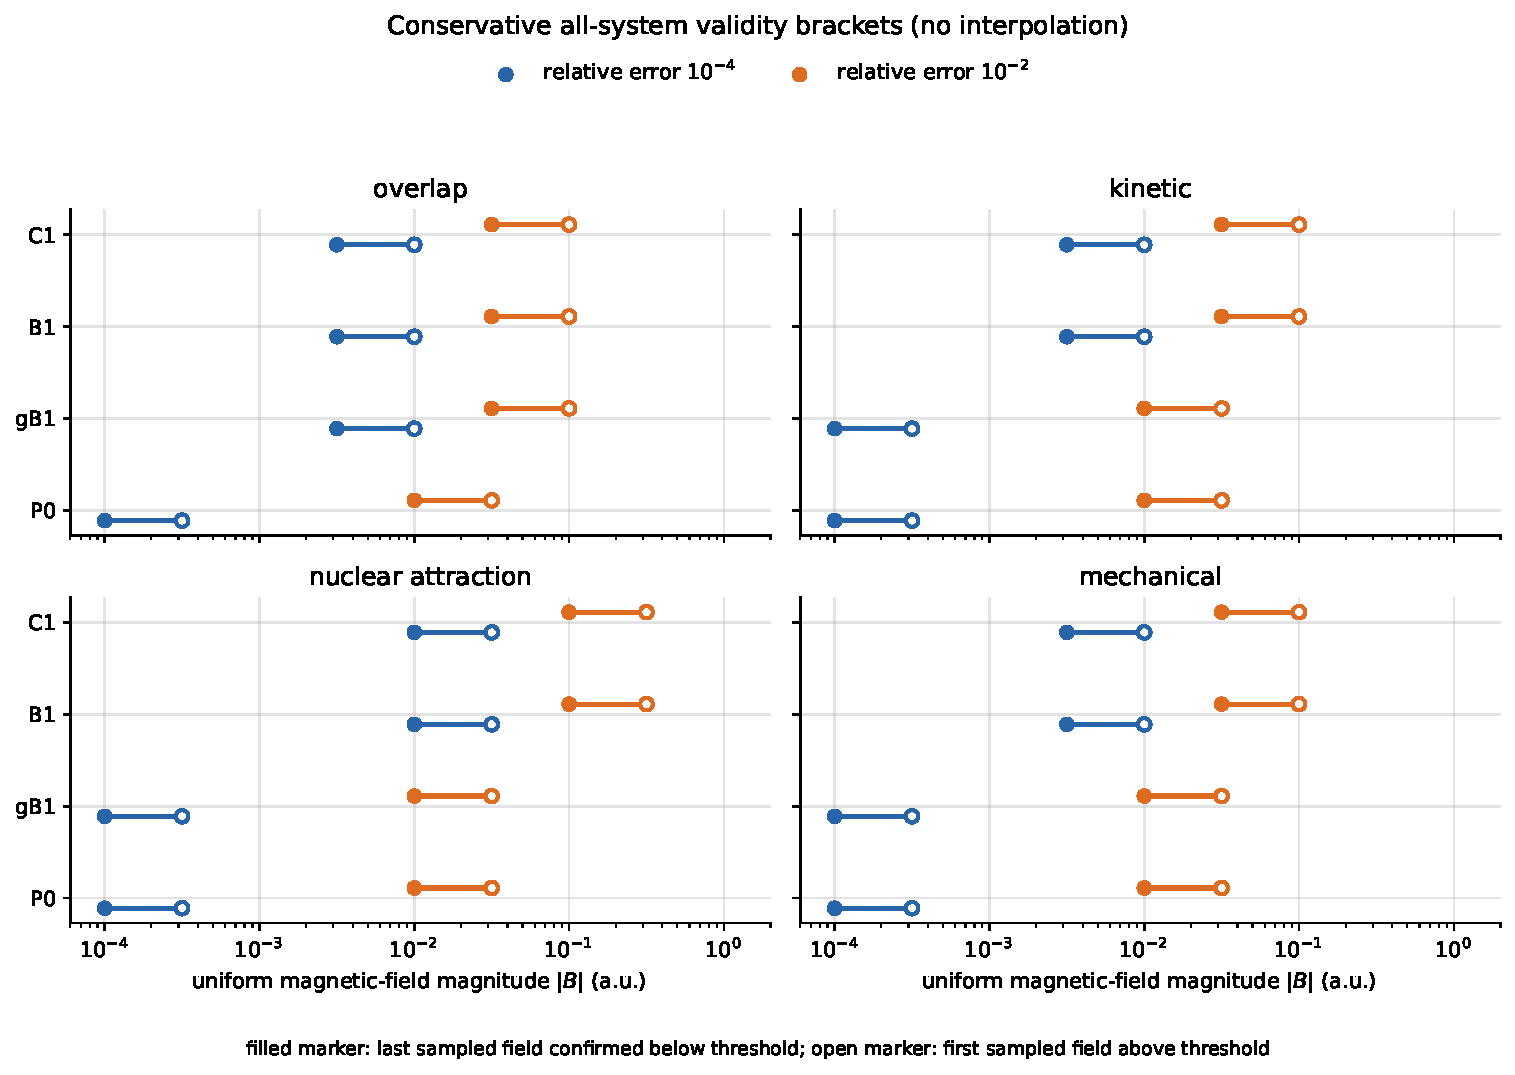
\includegraphics[width=\textwidth]{figures/exact_one_electron_qualification/global_validity_brackets.pdf}
\caption{Conservative all-system scan brackets from the authenticated WP8
synthesis.  A filled point is the last sampled field below the indicated
relative-error threshold; an open point is the first sampled field above it.
The segment is a bracket, not an interpolated transition.}
\label{fig:validity-brackets}
\end{figure}

The finite-field fits in Figure~\ref{fig:remainder-orders} show the intended
hierarchy: P0 errors are first order where the first internal amplitude is
missing; gB1 is second order only for overlap; B1 and C1 are second order for
all static magnetic matrix families.  C1 equals B1 here because the static
electric sector is absent.

\begin{figure}[htbp]
\centering
\includegraphics[width=0.94\textwidth]{/home/cgs/00_WORK/Projection_Code/CALCULATIONS/campaigns/exact_one_electron_qualification/wp4_first_order_20260918T191425Z_3fd2a83b77d1/analysis/figures/model_remainder_orders.pdf}
\caption{Observed finite-field remainder orders in the WP4 pair campaign.
The analytic first-order models remove the corresponding linear term, leaving
a quadratic remainder in their declared sectors.}
\label{fig:remainder-orders}
\end{figure}

The resolved mechanical audit finds 1,502 blocks that require the anchored-
vector B1 contribution: 372 onsite and 1,130 offsite.  Across angular blocks,
the minimum, median, and maximum B1 error-reduction factors are 11.65, 183.10,
and 868.36.  The independent uniform-electric E1 coefficient agrees with its
exact parent to $1.36\times10^{-14}$; the largest level-5 position-quadrature
relative residual is $7.36\times10^{-7}$.

\section{Multicentre loop flux and spectra: G5}

Two three-proton geometries, two basis sets, and sub-, near-, and
above-threshold positive-metric fields test the feature absent from a single
pair: a nonzero centre-loop holonomy.  The exact gauge-spectrum residual is at
most $5.80\times10^{-15}$ Ha and the loop identity residual is at most
$8.67\times10^{-16}$.  No metric regularization is used.

At the above-threshold cc-pVDZ point, the distorted geometry gives maximum
generalized-eigenvalue shifts of 14.203 Ha (P0), 1.0509 Ha (gB1), and
0.04216 Ha (B1/C1).  The associated largest subspace angles are approximately
$\pi/2$, $\pi/2$, and 0.02590 rad.  The equilateral values are 18.260 Ha,
1.6768 Ha, and 0.03184 Ha, with B1/C1 subspace angle 0.00656 rad.
Figure~\ref{fig:multicentre-spectra} shows the complete selected-field trend.

\begin{figure}[htbp]
\centering
\includegraphics[width=0.92\textwidth]{/home/cgs/00_WORK/Projection_Code/CALCULATIONS/campaigns/exact_one_electron_qualification/wp5_multicentre_20260918T200808Z_3fd2a83b77d1/analysis/figures/generalized_spectral_shifts.pdf}
\caption{Maximum generalized-eigenvalue shifts relative to EX in the
multicentre campaign.  The cc-pVDZ panels resolve the strong loop-flux failure
of P0/gB1 and the improvement from the full B1 mechanical response.}
\label{fig:multicentre-spectra}
\end{figure}

\section{Time-dependent source and connection}

For a uniform time-dependent magnetic field, the symmetric representative is
\begin{equation}
 \A_{\rm sym}(\rvec,t)=\tfrac12\B(t)\times(\rvec-\mathbf o),
 \qquad
 \Phi_{\rm sym}(\rvec,t)=-\E_{\mathbf o}(t)\cdot(\rvec-\mathbf o).
\end{equation}
It produces
\begin{equation}
 \E(\rvec,t)=\E_{\mathbf o}(t)
 +\tfrac12(\rvec-\mathbf o)\times\dot{\B}(t).
\end{equation}
The affine induction term is compulsory when $\dot{\B}\ne0$.  Landau gauge
adds the corresponding $-\partial_t\lambda$ to the scalar potential, so both
representatives describe the same $\E$ and $\B$.

The exact endpoint-factorized connection is evaluated independently of a
direct-grid differentiation of the ket Wilson factor.  The metric rate is
assembled by differentiating both the endpoint link and triangle factor, then
checked against both $\omega_t+\omega_t^\dagger$ and a central finite
difference of independently evaluated static metrics.  The connection is
therefore known analytically at every requested source time; no auxiliary ODE
for $S$ or $\omega_t$ is integrated.

\section{Time integration: exploration and accepted algorithm}

\subsection{Why the original checkpoint failed}

The original WP6 checkpoint evaluated one complete EOM triple at each
midpoint, advanced coefficients with a diagonal $[2/2]$ Pad\'e step, and
applied a right-Cholesky endpoint correction.  Its 8/16/32 supplement showed
second-order trajectory convergence (minimum measured order 1.9855), good
norm and metric-compatibility residuals, and a positive metric.  Nevertheless,
the maximum 16-to-32 change in a model-minus-exact density difference was
3.338 times the final difference, above the predeclared 0.25 limit.

This was not evidence that $S$ became singular: the minimum metric eigenvalue
was $6.54\times10^{-3}$.  It showed that the observable used to compare
models was still dominated by propagation error.  The result is preserved as
failed scientific evidence rather than hidden or reclassified.

\subsection{Mixed-index geometry}

Define the natural mixed density
\begin{equation}
 D^\mu{}_{\nu}=P^{\mu\lambda}S_{\lambda\nu}=PS.
\end{equation}
With
\begin{equation}
 G=S^{-1}\left(-\omega_t-\frac{\iu}{\hbar}K\right),
\end{equation}
metric compatibility converts the contravariant-density equation into
\begin{equation}
 \boxed{\dot D=[G,D].}
\end{equation}
If $U$ solves $\dot U=GU$, then
\begin{equation}
 D(t_1)=U(t_1,t_0)D(t_0)U(t_1,t_0)^{-1}.
\end{equation}
The similarity update preserves trace, eigenvalues, and $D^2=D$
algebraically.  Physical Hermiticity is $D^\dagger S=SD$.  The contravariant
density is recovered by solving $P=DS^{-1}$, without forming an explicit
inverse.

This is the geometric simplification: the time-dependent metric has not
vanished, but its connection is contained in the complete generator $G$, and
the mixed-index object evolves by a standard similarity commutator.

\subsection{Fourth-order Gauss--Magnus and diagonal Pad\'e link}

For a step $h$, evaluate the complete generator at
\begin{equation}
 t_\pm=t_n+\left(\frac12\pm\frac{\sqrt3}{6}\right)h.
\end{equation}
The fourth-order Magnus exponent is
\begin{equation}
 \Omega_4=\frac h2(G_-+G_+)
 -\frac{\sqrt3h^2}{12}[G_-,G_+].
\end{equation}
The transport link is the diagonal Pad\'e approximation
\begin{equation}
 U_n=R_{22}(\Omega_4)
 =\left(I-\frac{\Omega_4}{2}+\frac{\Omega_4^2}{12}\right)^{-1}
  \left(I+\frac{\Omega_4}{2}+\frac{\Omega_4^2}{12}\right).
\end{equation}
Its truncation begins at fifth order and therefore does not lower the formal
fourth order of the Magnus step.  The accepted update is
$D_{n+1}=U_nD_nU_n^{-1}$.

There is no orthogonalization, endpoint Cholesky factor, or metric correction.
Instead Aion records the raw cross-metric defect
\begin{equation}
 U_n^\dagger S(t_{n+1})U_n-S(t_n),
\end{equation}
as well as trace, idempotency, mixed metric-Hermiticity, recovered-$P$
Hermiticity, generator norms, and generator commutators.  The current API is
named \texttt{Experimental} because it consumes a prequalified linear history;
the self-consistent nonlinear Gauss-node solve is not yet implemented.

\subsection{Accepted convergence and stability}

The targeted 32/64/128 continuation of the hardest selected fixture gives
global orders 3.978 (EX), 3.707 (P0), 3.716 (E1), 3.986 (gB1), 3.990 (B1),
and 3.978 (C1).  P0 and E1 require finer steps because their approximate
generators are larger and more strongly noncommuting; the eventual
fourth-order regime demonstrates a pre-asymptotic timestep effect, not a
failure of the mixed-index equation.

\begin{figure}[htbp]
\centering
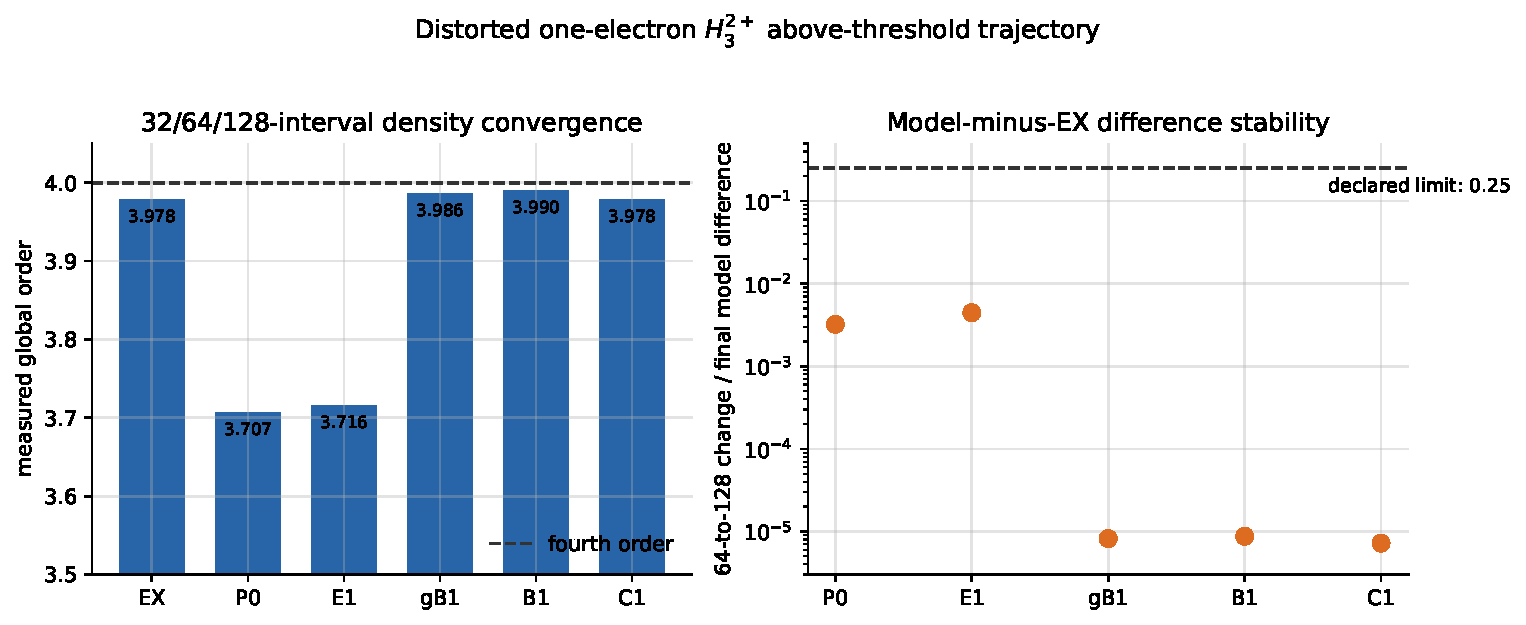
\includegraphics[width=\textwidth]{figures/exact_one_electron_qualification/temporal_convergence_and_stability.pdf}
\caption{Final hard-case convergence evidence.  The left panel isolates the
32/64/128 measured order for each model.  The right panel compares the
64-to-128 change in each model-minus-EX density difference with the declared
0.25 stability limit.}
\label{fig:temporal-convergence}
\end{figure}

Across the accepted continuation, trace drift is below
$6.7\times10^{-16}$, the idempotency residual below $5.5\times10^{-15}$,
and the minimum metric eigenvalue is $6.536\times10^{-3}$.

\section{Dynamic model comparison: G6}

The distorted above-threshold pulse has duration 4 a.u. and peak centre-loop
flux 0.05 a.u.  It simultaneously activates the electric and magnetic
finite-spread sectors.  The field returns to the declared endpoint, so the
reported endpoint energy is evaluated with the common field-free mechanical
operator.

At 128 intervals ($\Delta t=0.03125$ a.u.), EX absorbs
$2.805397\times10^{-5}$ Ha.  The approximate values are
$1.781478\times10^{-4}$ (P0), $1.885249\times10^{-4}$ (E1),
$4.921313\times10^{-4}$ (gB1), $1.706561\times10^{-4}$ (B1), and
$2.783231\times10^{-5}$ Ha (C1).  The exact excitation probability is
$2.199458\times10^{-5}$ and C1 gives $2.189968\times10^{-5}$.

The endpoint metric Hilbert--Schmidt density distances from EX are 0.01428
(P0), 0.01025 (E1), 0.02391 (gB1), 0.01457 (B1), and
$8.8254\times10^{-4}$ (C1).  Figure~\ref{fig:endpoint-observables} shows that
the observables have stabilized over 16--128 intervals; Figure
\ref{fig:dynamic-resolution} places the final physical separation beside the
64-to-128 difference uncertainty.

\begin{figure}[htbp]
\centering
\includegraphics[width=\textwidth]{/home/cgs/00_WORK/Projection_Code/CALCULATIONS/campaigns/exact_one_electron_qualification/wp6_mixed_magnus_n128_diagnostics_20260919T124656Z_73f6dc1cb760/endpoint_observables/endpoint_observables.pdf}
\caption{Field-free endpoint observables for the distorted one-electron
$\mathrm H_3^{2+}$ above-threshold pulse.  C1 is the only tested first-order
model that remains close to EX in all three panels.}
\label{fig:endpoint-observables}
\end{figure}

\begin{figure}[htbp]
\centering
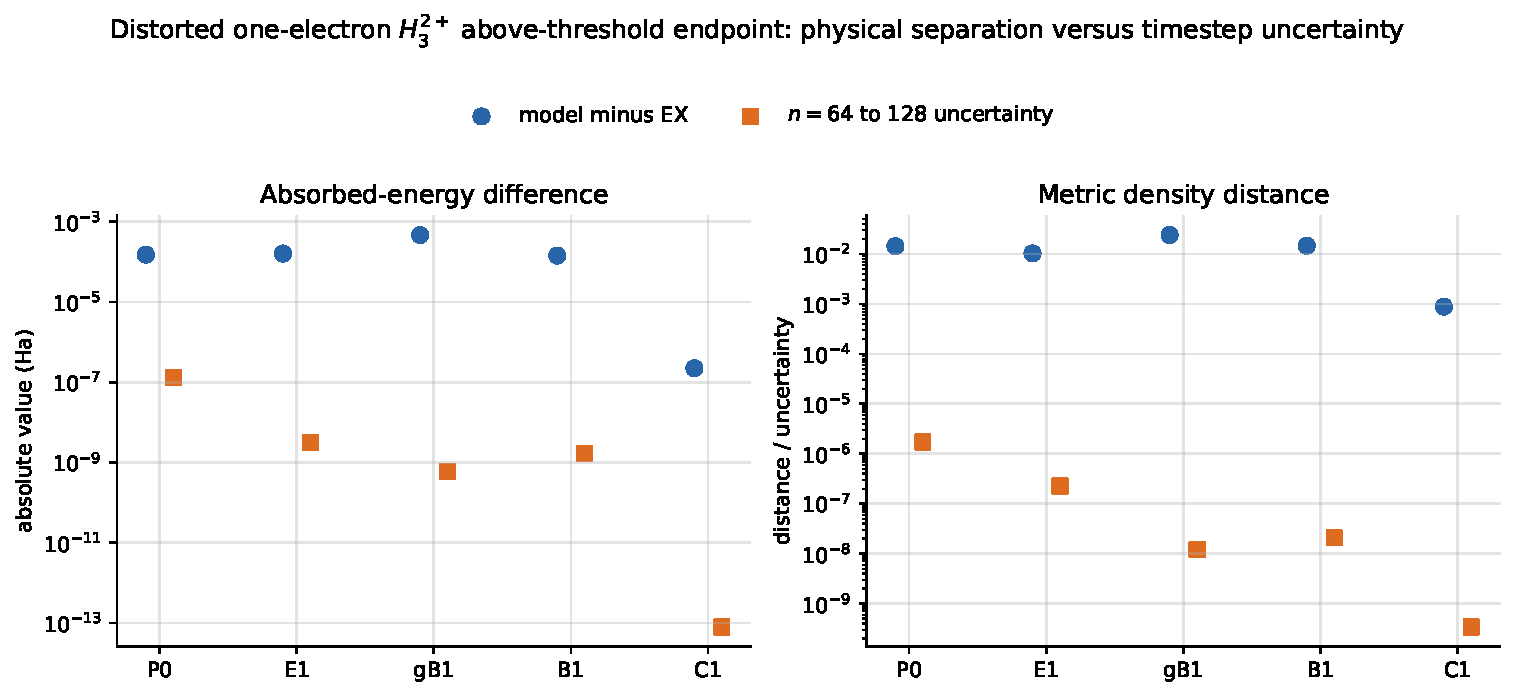
\includegraphics[width=\textwidth]{figures/exact_one_electron_qualification/dynamic_difference_resolution.pdf}
\caption{Absolute model-minus-EX endpoint differences compared directly with
their 64-to-128 timestep difference uncertainty.  The many-decade separation
for C1 establishes a resolved truncation error rather than a time-integration
artifact.}
\label{fig:dynamic-resolution}
\end{figure}

The physical conclusion is not that B1 ``fails'' generally.  It is that a
magnetic-only first-order model cannot reproduce a trajectory that also
contains the internal electric E1 response.  Conversely, E1 has the electric
sector but omits the magnetic metric and mechanical sectors.  C1 contains
both at the same action level.

\section{Action observables, continuity, and power: G7}

\subsection{Variational source directions}

For fixed coefficient history, a real source parameter $\lambda$ with matrix
directions $(S_\lambda,K_\lambda,\omega_\lambda)$ gives the implemented
instantaneous action derivative
\begin{equation}
 \frac{\partial L}{\partial\lambda}\bigg|_{C,\dot C}
 =\Re\left\{
 \frac{\iu\hbar}{2}\Tr[(R-R^\dagger)S_\lambda
 +P(\omega_\lambda-\omega_\lambda^\dagger)]
 -\Tr(PK_\lambda)\right\},
\end{equation}
where $R=\dot C fC^\dagger=GP$ on shell.  Aion separately exposes the metric
kinematic, connection kinematic, and mechanical contributions.  Currents are
therefore derivatives of the same restricted action used for propagation,
not ambient momentum expectations borrowed from another model.

The implemented directions include independent anchor scalar potentials,
oriented endpoint links, complete instantaneous uniform $\B$, separated
endpoint/internal magnetic parts, pure-gauge source/history pairs, uniform
electric components, and localized Gaussian vector-potential variations.
Site charges and oriented pair currents obey the declared incidence
convention $\dot Q+\mathcal I I=0$.

The projected ambient mechanical current remains a useful diagnostic, but in
a finite source-dependent subspace it need not equal the variational source
current.  Their difference measures finite-subspace and source-response
effects; it is not automatically an implementation error.

\subsection{Uniform-electric power}

In the zero-$B$ specialization the three electric-field action derivatives
define the electronic polarization.  Applying the same covectors to $\dot P$
defines $\mathbf J_{\rm src}$ and yields
\begin{equation}
 \frac{\dd U}{\dd t}=\E(t)\cdot\mathbf J_{\rm src}(t).
\end{equation}
No momentum operator is inserted into this identity.  The finest
$\Delta t=0.125$ a.u. trajectory has maximum instantaneous power residual
$4.88\times10^{-16}$, while the integrated work defect is
$-1.236\times10^{-9}$ Ha.  The difference is expected: instantaneous source
contraction is algebraic, whereas accumulated work and a centred trajectory
derivative carry fourth- and second-order time-discretization errors,
respectively.

\begin{figure}[htbp]
\centering
\includegraphics[width=0.82\textwidth]{/home/cgs/00_WORK/Projection_Code/CALCULATIONS/campaigns/exact_one_electron_qualification/wp7_observables_cpu_20260919T145221Z_7d603105e1db/analysis/figures/electric_power_history.png}
\caption{Uniform-electric exact-Wilson trajectory.  The upper panel compares
mechanical-energy change with integrated source work.  The lower panel
separates the roundoff-level instantaneous action identity from the expected
finite-difference trajectory derivative error.}
\label{fig:electric-power}
\end{figure}

\begin{figure}[htbp]
\centering
\includegraphics[width=\textwidth]{/home/cgs/00_WORK/Projection_Code/CALCULATIONS/campaigns/exact_one_electron_qualification/wp7_observables_cpu_20260919T145221Z_7d603105e1db/analysis/figures/observable_refinement.png}
\caption{WP7 refinement summary.  Integrated power balance converges at
fourth order, the centred trajectory derivative at second order, and the
continuity, Ward, and charge identities remain near roundoff.}
\label{fig:observable-refinement}
\end{figure}

Measured integrated-work orders are 3.9658 and 3.9914; centred derivative
orders are 1.9464 and 1.9931.  At the finest electric step, the maximum
continuity, Ward, and total-charge residuals are $2.57\times10^{-15}$,
$3.89\times10^{-16}$, and $1.22\times10^{-15}$.

\subsection{Magnetic identities and GPU parity}

For the finest magnetic trajectory, the maximum cross-metric residual is
$3.30\times10^{-12}$; continuity, Ward, and total-charge residuals are
$3.93\times10^{-15}$, $4.44\times10^{-16}$, and $6.66\times10^{-16}$.
Figure~\ref{fig:magnetic-identities} shows their history.

\begin{figure}[htbp]
\centering
\includegraphics[width=0.82\textwidth]{/home/cgs/00_WORK/Projection_Code/CALCULATIONS/campaigns/exact_one_electron_qualification/wp7_observables_cpu_20260919T145221Z_7d603105e1db/analysis/figures/magnetic_identity_history.png}
\caption{Action-derived local continuity, pure-gauge Ward, and total-charge
residuals on the finest time-dependent magnetic trajectory.}
\label{fig:magnetic-identities}
\end{figure}

The physical-GPU n=32 comparison gives maximum CPU/GPU absolute differences
of $1.94\times10^{-15}$ (electric density), $3.18\times10^{-15}$ (electric
diagnostics), $1.53\times10^{-15}$ (magnetic density), and
$4.14\times10^{-15}$ (magnetic diagnostics).  The final fast CPU suite before
G8 reported 88 passes and 133 deselections; targeted physical-GPU tests were
also executed and accepted.

\section{G8 synthesis, accepted boundary, and next branch}

The WP8 synthesis authenticates the accepted G3--G7 records and produces five
compact tables:

\begin{itemize}
  \item 768 system/basis-specific magnetic validity rows;
  \item 64 conservative global validity rows;
  \item 10 mechanical channel-attribution rows;
  \item 48 multicentre spectral-comparison rows; and
  \item 5 dynamic endpoint-difference rows.
\end{itemize}

G8 was explicitly accepted.  The bounded validity statement is:

\begin{quote}
The fixed-centre linear exact one-electron Wilson dynamics and its P0, E1,
gB1, B1, and C1 truncations are qualified only over the explicitly tabulated
systems, bases, geometries, fields, source histories, quadrature levels, and
timesteps.  The reported ranges are scan brackets and every physical
comparison retains its quadrature or timestep companion.
\end{quote}

The accepted post-G8 choice is \emph{Aion adiabatic pure-LDA/GGA TDDFT
closure}.  This follows from the measured boundary: source-only exact Wilson
geometry, connection-aware linear propagation, action source derivatives,
and CPU/GPU parity now have accepted evidence, while self-consistent
Hartree/XC response and nonlinear Gauss-node propagation do not.  This report
does not plan or implement that branch; it closes and indexes the evidence on
which the branch choice rests.

\clearpage
\appendix

\section{Authoritative documents}\label{sec:document-index}

The mathematical authority and operational plan are outside the Aion
worktree; implementation notes and review decisions are versioned with the
code.  The following links are intended as the reading order.

\begin{enumerate}
  \item \filelink{Wilson-dressed adiabatic TDDFT reference (TeX)}{/home/cgs/00_WORK/Projection_Full_Formalism/REVIEW/implementation/wilson_dressed_adiabatic_tddft_reference.tex} --- complete fixed-centre action, density, XC/RI-Hartree closure target, source derivatives, and staged realization.
  \item \filelink{Wilson-dressed adiabatic TDDFT reference (PDF)}{/home/cgs/00_WORK/Projection_Full_Formalism/REVIEW/implementation/wilson_dressed_adiabatic_tddft_reference.pdf}.
  \item \filelink{Exact one-electron numerical qualification plan}{/home/cgs/00_WORK/Projection_Full_Formalism/REVIEW/implementation/exact_one_electron_numerical_qualification_plan.md} --- gate definitions and original acceptance criteria.  Its embedded status table is historical; the review records below are authoritative for final gate state.
  \item \filelink{Exact one-electron qualification agent brief}{/home/cgs/00_WORK/Projection_Full_Formalism/REVIEW/implementation/aion_exact_one_electron_qualification_agent_prompt.md} --- execution discipline and evidence-status contract used for the campaign.
  \item \filelink{Exact Wilson matrix-element qualification note (TeX)}{/home/cgs/00_WORK/Projection_Full_Formalism/REVIEW/implementation/exact_wilson_matrix_element_qualification.tex} and \filelink{PDF}{/home/cgs/00_WORK/Projection_Full_Formalism/REVIEW/implementation/exact_wilson_matrix_element_qualification.pdf}.
  \item \filelink{G0 conventions and schema note}{/home/cgs/00_WORK/Projection_Code/aion-magnetic-matrix-benchmark/docs/exact_one_electron_qualification_g0.md}.
  \item \filelink{WP1 overlap/kinetic checkpoint}{/home/cgs/00_WORK/Projection_Code/aion-magnetic-matrix-benchmark/docs/exact_one_electron_wp1_overlap_kinetic_checkpoint.md} and \filelink{WP1 zero-field qualification}{/home/cgs/00_WORK/Projection_Code/aion-magnetic-matrix-benchmark/docs/exact_one_electron_wp1_zero_field_qualification.md}.
  \item \filelink{WP2 static Wilson qualification}{/home/cgs/00_WORK/Projection_Code/aion-magnetic-matrix-benchmark/docs/exact_one_electron_wp2_static_wilson_qualification.md}.
  \item \filelink{WP6 time connection and linear propagation}{/home/cgs/00_WORK/Projection_Code/aion-magnetic-matrix-benchmark/docs/exact_one_electron_wp6_time_connection_linear_propagation.md}.
  \item \filelink{Mixed-density Gauss--Magnus experiment}{/home/cgs/00_WORK/Projection_Code/aion-magnetic-matrix-benchmark/docs/experimental_wp6_mixed_density_magnus.md}.
  \item \filelink{WP8 synthesis narrative}{/home/cgs/00_WORK/Projection_Code/CALCULATIONS/campaigns/exact_one_electron_qualification/wp8_synthesis_20260919T152644Z_2fa0214fa659/synthesis.md}.
\end{enumerate}

Related general Aion documents are:
\begin{itemize}
  \item \filelink{theory and implementation}{/home/cgs/00_WORK/Projection_Code/aion-magnetic-matrix-benchmark/docs/theory_and_implementation.tex};
  \item \filelink{user guide}{/home/cgs/00_WORK/Projection_Code/aion-magnetic-matrix-benchmark/docs/user_guide.md};
  \item \filelink{configuration and schema contracts}{/home/cgs/00_WORK/Projection_Code/aion-magnetic-matrix-benchmark/docs/configuration_and_schema_contracts.md}; and
  \item \filelink{magnetic benchmark API}{/home/cgs/00_WORK/Projection_Code/aion-magnetic-matrix-benchmark/docs/magnetic_benchmark_api.md}.
  \item \filelink{magnetic-matrix benchmark theory}{/home/cgs/00_WORK/Projection_Code/aion-magnetic-matrix-benchmark/docs/magnetic_matrix_benchmark_theory.tex};
  \item \filelink{magnetic-matrix benchmark contract}{/home/cgs/00_WORK/Projection_Code/aion-magnetic-matrix-benchmark/docs/magnetic_matrix_benchmark_contract.md};
  \item \filelink{magnetic-matrix benchmark implementation plan}{/home/cgs/00_WORK/Projection_Code/aion-magnetic-matrix-benchmark/docs/magnetic_matrix_benchmark_implementation_plan.md}; and
  \item \filelink{Aion refactor implementation plan}{/home/cgs/00_WORK/Projection_Code/aion-magnetic-matrix-benchmark/docs/refactor_implementation_plan.md}.
\end{itemize}

\section{Gate review records}\label{sec:review-index}

\begin{longtable}{llp{0.56\textwidth}}
\toprule
Gate & Decision & Record \\
\midrule
\endfirsthead
\toprule Gate & Decision & Record \\
\midrule
\endhead
G0 & accepted & \filelink{G0 review}{/home/cgs/00_WORK/Projection_Code/aion-magnetic-matrix-benchmark/docs/reviews/exact_one_electron_g0_review_20260916.json} \\
G1 & accepted & \filelink{G1 review}{/home/cgs/00_WORK/Projection_Code/aion-magnetic-matrix-benchmark/docs/reviews/exact_one_electron_g1_review_20260916.json} \\
G2 & accepted & \filelink{G2 review}{/home/cgs/00_WORK/Projection_Code/aion-magnetic-matrix-benchmark/docs/reviews/exact_one_electron_g2_review_20260916.json} \\
G3 & accepted & \filelink{G3 review}{/home/cgs/00_WORK/Projection_Code/aion-magnetic-matrix-benchmark/docs/reviews/exact_one_electron_g3_review_20260918.json} \\
G4 & accepted & \filelink{G4 review}{/home/cgs/00_WORK/Projection_Code/aion-magnetic-matrix-benchmark/docs/reviews/exact_one_electron_g4_review_20260918.json} \\
G5 & accepted & \filelink{G5 review}{/home/cgs/00_WORK/Projection_Code/aion-magnetic-matrix-benchmark/docs/reviews/exact_one_electron_g5_review_20260918.json} \\
G6 & accepted & \filelink{G6 review}{/home/cgs/00_WORK/Projection_Code/aion-magnetic-matrix-benchmark/docs/reviews/exact_one_electron_g6_review_20260919.json} \\
G7 & accepted & \filelink{G7 review}{/home/cgs/00_WORK/Projection_Code/aion-magnetic-matrix-benchmark/docs/reviews/exact_one_electron_g7_review_20260919.json}; the preserved \filelink{candidate}{/home/cgs/00_WORK/Projection_Code/aion-magnetic-matrix-benchmark/docs/reviews/exact_one_electron_g7_review_candidate_20260919.json} is pre-decision evidence. \\
G8 & accepted & \filelink{G8 review}{/home/cgs/00_WORK/Projection_Code/aion-magnetic-matrix-benchmark/docs/reviews/exact_one_electron_g8_review_20260919.json}; the preserved \filelink{candidate}{/home/cgs/00_WORK/Projection_Code/aion-magnetic-matrix-benchmark/docs/reviews/exact_one_electron_g8_review_candidate_20260919.json} contains the pre-decision synthesis and recommendation. \\
\bottomrule
\end{longtable}

\section{Campaign directory index}\label{sec:campaign-index}

All roots below live under
\path{/home/cgs/00_WORK/Projection_Code/CALCULATIONS/campaigns/exact_one_electron_qualification}.
The sizes are approximate and help identify the heavy raw data.  The accepted
roots are identified by the review records; historical and failed executions
remain part of the audit trail.

\small
\begin{longtable}{>{\raggedright\arraybackslash}p{0.37\textwidth}>{\raggedright\arraybackslash}p{0.12\textwidth}>{\raggedright\arraybackslash}p{0.43\textwidth}}
\toprule
Directory & Size/files & Purpose and status \\
\midrule
\endfirsthead
\toprule Directory & Size/files & Purpose and status \\
\midrule
\endhead
\path{20260916T184521Z_3fd2a83b77d1} & 3.4 MB / 17 & Initial G0 checkpoint execution retained as historical duplicate/restart; not the accepted root. \\
\path{20260916T184810Z_3fd2a83b77d1} & 3.4 MB / 17 & Accepted G0 H--H overlap/kinetic checkpoint; inspect \path{execution_index.json}. \\
\path{wp1_20260916T190311Z_3fd2a83b77d1} & 24 MB / 74 & Initial full WP1 execution retained as historical duplicate/restart. \\
\path{wp1_20260916T190346Z_3fd2a83b77d1} & 24 MB / 74 & Accepted G1 zero-field campaign; \path{execution_index.json} is the entry point. \\
\path{wp2_20260916T192437Z_3fd2a83b77d1} & 6.6 MB / 5 & Accepted G2 exact static Wilson evaluator/covariance campaign; \path{manifest.json}, \path{result.json}, \path{arrays.npz}. \\
\path{wp3_pair_20260916T195452Z_3fd2a83b77d1} & 1.9 MB / 4 & Initial WP3 pair-scan start retained for provenance; superseded by the complete scan. \\
\path{wp3_pair_20260916T195529Z_3fd2a83b77d1} & 531 MB / 76 & Complete reference-distance pair scan and its first analysis; figures/tables are under \path{analysis}. \\
\path{wp3_pair_distance_20260917T002456Z_3fd2a83b77d1} & 1.1 GB / 123 & Accepted G3 distance-complete pair campaign; combined entry point is \path{g3_analysis/report.md}. \\
\path{wp4_first_order_20260918T191425Z_3fd2a83b77d1} & 35 MB / 167 & Accepted G4 analytic first-order hierarchy, channel classification, and E1 audit; use \path{analysis/report.md}. \\
\path{wp5_multicentre_20260918T200808Z_3fd2a83b77d1} & 11 MB / 34 & Accepted G5 loop-flux, metric-domain, generalized-spectrum, and selected-dynamics cases; use \path{analysis/report.md}. \\
\path{wp6_linear_20260918T204830Z_3fd2a83b77d1} & 328 KB / 5 & Smoke run; \path{completed.json} says \status{smoke\_not\_qualification}. \\
\path{wp6_linear_20260918T205152Z_3fd2a83b77d1} & 356 KB / 5 & Second smoke run; \status{smoke\_not\_qualification}. \\
\path{wp6_linear_qualification_20260918T2055Z_3fd2a83b77d1} & 2.0 MB / 29 & Full initial midpoint/Cholesky qualification.  Important source evidence, but its model-difference stability was unresolved. \\
\path{wp6_h3_timestep_refinement_20260918T212428Z_3fd2a83b77d1} & 1.8 MB / 22 & Authenticated 8/16/32 supplement: second-order convergence, failed 0.25 model-difference stability criterion. \\
\path{wp6_mixed_magnus_20260918T231057Z_38ce83eb2fe9} & 16 MB / 16 & Replacement mixed-index Gauss--Magnus experiment and derived convergence/stability analysis. \\
\path{wp6_mixed_magnus_n64_20260919T120325Z_57ef2fb6d40e} & 3.0 MB / 10 & Targeted 64-interval continuation and endpoint observables. \\
\path{wp6_mixed_magnus_n128_diagnostics_20260919T124656Z_73f6dc1cb760} & 5.7 MB / 10 & Accepted hard-case 128-interval continuation, full diagnostics, convergence, stability, and endpoint observables. \\
\path{wp7_observables_cpu_20260919T145221Z_7d603105e1db} & 496 KB / 10 & Accepted CPU action-observable histories, refinement table, figures, and summary. \\
\path{wp7_observables_gpu_20260919T145459Z_7d603105e1db} & 28 KB / 5 & Accepted physical-CuPy parity execution. \\
\path{wp8_synthesis_20260919T152644Z_2fa0214fa659} & 208 KB / 9 & Authenticated G8 synthesis, five compact tables, summary, manifest, and narrative. \\
\bottomrule
\end{longtable}
\normalsize

\section{Derived tables and figures}\label{sec:derived-index}

The compact final tables are:

\begin{itemize}
  \item \filelink{magnetic validity by system and basis}{/home/cgs/00_WORK/Projection_Code/CALCULATIONS/campaigns/exact_one_electron_qualification/wp8_synthesis_20260919T152644Z_2fa0214fa659/tables/magnetic_validity_by_system_basis.csv};
  \item \filelink{global magnetic validity}{/home/cgs/00_WORK/Projection_Code/CALCULATIONS/campaigns/exact_one_electron_qualification/wp8_synthesis_20260919T152644Z_2fa0214fa659/tables/magnetic_validity_global.csv};
  \item \filelink{channel attribution}{/home/cgs/00_WORK/Projection_Code/CALCULATIONS/campaigns/exact_one_electron_qualification/wp8_synthesis_20260919T152644Z_2fa0214fa659/tables/channel_attribution.csv};
  \item \filelink{multicentre spectral differences}{/home/cgs/00_WORK/Projection_Code/CALCULATIONS/campaigns/exact_one_electron_qualification/wp8_synthesis_20260919T152644Z_2fa0214fa659/tables/multicentre_spectral_differences.csv}; and
  \item \filelink{dynamic endpoint differences}{/home/cgs/00_WORK/Projection_Code/CALCULATIONS/campaigns/exact_one_electron_qualification/wp8_synthesis_20260919T152644Z_2fa0214fa659/tables/dynamic_endpoint_differences.csv}.
\end{itemize}

The most useful gate-specific derived roots are:

\begin{itemize}
  \item \filelink{G3 combined analysis}{/home/cgs/00_WORK/Projection_Code/CALCULATIONS/campaigns/exact_one_electron_qualification/wp3_pair_distance_20260917T002456Z_3fd2a83b77d1/g3_analysis};
  \item \filelink{G4 analysis}{/home/cgs/00_WORK/Projection_Code/CALCULATIONS/campaigns/exact_one_electron_qualification/wp4_first_order_20260918T191425Z_3fd2a83b77d1/analysis};
  \item \filelink{G5 analysis}{/home/cgs/00_WORK/Projection_Code/CALCULATIONS/campaigns/exact_one_electron_qualification/wp5_multicentre_20260918T200808Z_3fd2a83b77d1/analysis};
  \item \filelink{failed midpoint supplement analysis}{/home/cgs/00_WORK/Projection_Code/CALCULATIONS/campaigns/exact_one_electron_qualification/wp6_h3_timestep_refinement_20260918T212428Z_3fd2a83b77d1/analysis};
  \item \filelink{mixed-Magnus analysis}{/home/cgs/00_WORK/Projection_Code/CALCULATIONS/campaigns/exact_one_electron_qualification/wp6_mixed_magnus_20260918T231057Z_38ce83eb2fe9/analysis};
  \item \filelink{128-interval endpoint observables}{/home/cgs/00_WORK/Projection_Code/CALCULATIONS/campaigns/exact_one_electron_qualification/wp6_mixed_magnus_n128_diagnostics_20260919T124656Z_73f6dc1cb760/endpoint_observables}; and
  \item \filelink{G7 observable analysis}{/home/cgs/00_WORK/Projection_Code/CALCULATIONS/campaigns/exact_one_electron_qualification/wp7_observables_cpu_20260919T145221Z_7d603105e1db/analysis}.
\end{itemize}

The report-specific figures in
\path{docs/figures/exact_one_electron_qualification} are regenerated by
\texttt{tools/build\_exact\_one\_electron\_qualification\_report\_assets.py}
from the authenticated WP8 tables and WP6 n=128 result.  They do not alter the
source evidence.

\section{Runner, analyzer, and verifier index}\label{sec:tool-index}

The campaign tools are grouped by role rather than copied into the scientific
API.

\begin{description}[style=nextline]
  \item[Run]
  \begin{itemize}
    \item \path{run_exact_one_electron_wp1_checkpoint.py}
    \item \path{run_exact_one_electron_wp1_full.py}
    \item \path{run_exact_one_electron_wp2.py}
    \item \path{run_exact_one_electron_wp3_pair_scan.py}
    \item \path{run_exact_one_electron_wp3_reference_audit.py}
    \item \path{run_exact_one_electron_wp4_first_order.py}
    \item \path{run_exact_one_electron_wp4_e1_audit.py}
    \item \path{run_exact_one_electron_wp5_multicentre.py}
    \item \path{run_exact_one_electron_wp6_linear.py}
    \item \path{run_exact_one_electron_wp6_h3_timestep_refinement.py}
    \item \path{run_exact_one_electron_wp6_mixed_magnus.py}
    \item \path{run_exact_one_electron_wp6_mixed_magnus_n64.py}
    \item \path{run_exact_one_electron_wp6_mixed_magnus_n128_diagnostics.py}
    \item \path{run_exact_one_electron_wp7_observables.py}
  \end{itemize}
  \item[Analyze]
  The correspondingly named \texttt{analyze\_exact\_one\_electron\_*}
  tools for G3, G4, G5, the WP6 primary/supplement/mixed/endpoint paths, G7,
  and G8.  \path{analyze_exact_one_electron_wp8_synthesis.py} is the
  final cross-gate reducer.
  \item[Verify]
  The correspondingly named \texttt{verify\_exact\_one\_electron\_*} tools
  independently recompute manifest identities, hashes, row counts, and
  declared residual decisions.  The WP8 verifier authenticates all five
  synthesis tables.
\end{description}

All are under
\path{/home/cgs/00_WORK/Projection_Code/aion-magnetic-matrix-benchmark/tools}.

\section{Fixtures and automated tests}\label{sec:test-index}

The immutable fixture directory is
\path{tests/fixtures/exact_one_electron}.  It contains H--H and O--H reference
fixtures, the G2 oblique regression, the WP3 pair campaign, the WP5
multicentre campaign, the WP6 linear/midpoint/mixed/n64/n128 declarations,
and the WP7 observables declaration.

The principal CPU tests are:
\begin{itemize}
  \item \path{tests/test_exact_one_electron_wp0_wp1.py}
  \item \path{tests/test_exact_one_electron_wp1_full.py}
  \item \path{tests/test_exact_one_electron_wp2.py}
  \item \path{tests/test_exact_one_electron_wp3_analysis.py}
  \item \path{tests/test_exact_one_electron_wp4.py}
  \item \path{tests/test_exact_one_electron_wp6.py}
  \item \path{tests/test_exact_one_electron_wp7.py}
  \item \path{tests/test_tensorial_magnus.py}
\end{itemize}
Physical-GPU tests are:
\begin{itemize}
  \item \path{tests/test_exact_one_electron_wp6_gpu.py}
  \item \path{tests/test_exact_one_electron_wp7_gpu.py}
  \item \path{tests/test_tensorial_magnus_gpu.py}
\end{itemize}

\section{Authentication anchors}

The accepted WP8 synthesis root has manifest ID
\begin{center}
\texttt{f41bbd648891028d9665caf13f5ab1801b46c8d87eb535db3a5471c0f88f41c8}.
\end{center}
Its principal SHA-256 values are:

\begin{center}\scriptsize
\begin{tabular}{ll}
\toprule
Artifact & SHA-256 \\
\midrule
\texttt{completed.json} & \texttt{da2de4de08498cbfe69ce12448f8dc28a5069bd2866d2dc6cc5b8630445bc72d} \\
\texttt{manifest.json} & \texttt{929ba2f569b824494f3a43c3fb1773d286f2ae818f1611b0e04fe20980420f81} \\
\texttt{summary.json} & \texttt{4c5cb2146cf63390424ec1c8aa28c1d39d5827f6d146169a9db80b646b9f662c} \\
\texttt{synthesis.md} & \texttt{e7f31b688e4e75f6e787828ecd073345fe6eafd98bca101129d52688d1ce8bc2} \\
\bottomrule
\end{tabular}
\end{center}

Earlier per-gate manifest IDs and SHA-256 anchors are retained in the G0--G7
review JSON records rather than duplicated here.  This ensures that future
edits to the narrative do not silently redefine the accepted raw evidence.

\end{document}
